\chapter{Introduction}
\label{chp:intro}

One of the most powerful and universally accepted rules in the philosophy of human behaviour is the 80/20 rule proposed by famous Italian economist, Vilfredo Pareto \cite{pareto1971}, stating:

\textit{For many events, roughly 80\% of the effects come from 20\% of the causes.}

This means that 80\% of the crimes in a society are committed by 20\% of the people; 20\% drivers cause 80\% of the accidents; and – of our interest – 80\% of the ideas, news and products are promoted in a society by 20\% of the people; 80\% of the global resources are consumed by 20\% countries.

This rule leads us to think in a new dimension to market our ideas, products and services; if we can target those 20\% of the people, we can approach the rest of 80\% without needing any additional budget and efforts. If a product is bought by 20\% people, it will automatically be propagated to the rest of the population.

Malcom Gladwell \cite{gladwell2006} writes in his famous best seller book, The tipping point:

\textit{There are exceptional people out there who are capable of starting epidemics. All you have to do is find them.}

An idea or a product can reach the tipping point (go viral/become popular/turn into an epidemic) in a society, in a very short period of time if we can inspire some exceptional/influential people from the society to adopt it; these exceptional people have the capability to inspire and spread a phenomena to everyone else. Often these individuals are collectively called super spreaders. The challenging question here is: How to find those exceptional people?

Thus, the broader question: "how to find  the most influential people, places, events, or simply put, find super spreaders?" is a holy grail for a variety of domains. This million dollar question has caught eyes of people keen to exploit the power of these individuals and cause a ripple effect on mass scale from sectors as diverse as social networks \cite{chen2009, bonchi2011}, technological networks \cite{wang2010,teuscher2006}, and ecological networks \cite{williams2002,guimaraes2007}. The next section introduces some of the real world examples that provide a very good understanding of how influential people, places or events can cause global impact.

	\section{Historic events with global reach}
	\label{sec:intro-global-events}
	History has observed many events where something considered as a common event sparked a reaction, which affected the world on a massive scale. Here are a few for appetite-whetting:
	
		\subsection{Eyjafjallajökull Volcano eruptions}	
		The famous 2010 eruptions of Eyjafjallajökull\footnote{Ei-ya-fyat-LA-yer-kitle} volcano in Iceland (see Figure \ref{fig:intro-eyjafjallajokull}) created a large cloud of ash which lead to the closure of most of the flights across and around Iceland for 6 days. As a consequence, the air travel industry faced its second biggest disruption after Word War 2 \cite{gudmundsson2010}. These eruptions were not the largest from a volcano but the strategic position of Iceland in the air transport industry resulted in this huge impact as the ashes from the volcano blocked the air space for all the flights passing over.
		
		\begin{figure}[h]
			\centering
			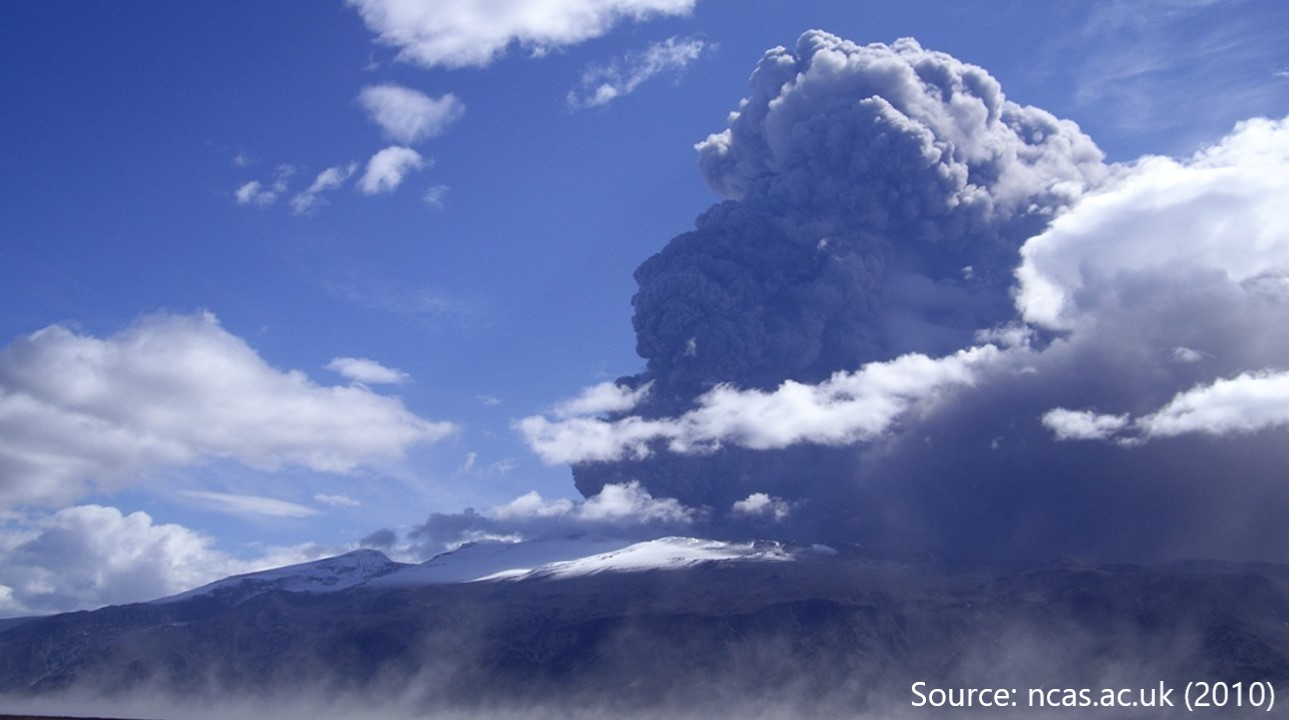
\includegraphics[width=1\textwidth]{eyjafjallajokull}
			\caption[Eruption from peaks of Eyjafjallajökull]{Eruption from peaks of Eyjafjallajökull - 2010. (Source ncas.ac.uk - 2010)}
			\label{fig:intro-eyjafjallajokull}
		\end{figure}
	
		\subsection{Northeast power outage in USA}
		In August of 2003, the northeastern part of USA faced a historical power outage, which affected 50 million consumers \cite{schewe2004}. The cause turned out to be no actual failure but an insignificant software bug that triggered a fail-safe alarm. The blackout would last two days in New York, New Jersey, Massachusetts, Michigan, and Ohio in USA, and in Ottawa and Toronto in Canada and the power disruption caused economic disturbance on a huge scale (see Figure \ref{fig:intro-northamerica-blackout}).
		
		\begin{figure}[h]
			\centering
			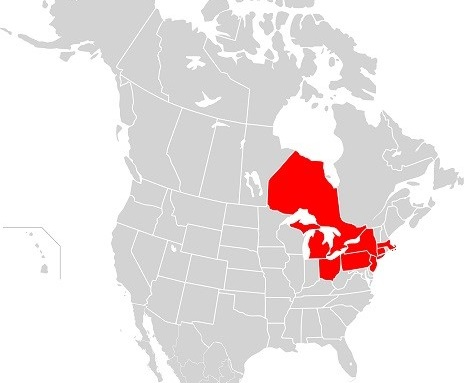
\includegraphics[width=1\textwidth]{northamerica-blackout}
			\caption[Northeast power outage]{Approximate area affected due to Northeast area power outage in 2003 (Source: Wikipedia - Lokal\_Profil).}
			\label{fig:intro-northamerica-blackout}
		\end{figure}

		\subsection{Suez canal blockage}
		In a recent incident, a 200 ton-heavy cargo vessel named Evergreen jammed in a small pass of Suez Canal, causing major disruption in global supplies of oil and other goods (See Figure \ref{fig:intro-evergreen-blockage}). The consequent financial loss incurred to the trade industry was estimated to be 400 million USD per hour for 6 days \footnote{Source: https://www.foxbusiness.com/markets/white-house-eyes-suez-canal-energy-impact}. In the global network of transport, the Suez canal is a tiny route but its significance is much higher than a majority of other channels in the world.
	
		\begin{figure}[H]
			\centering
			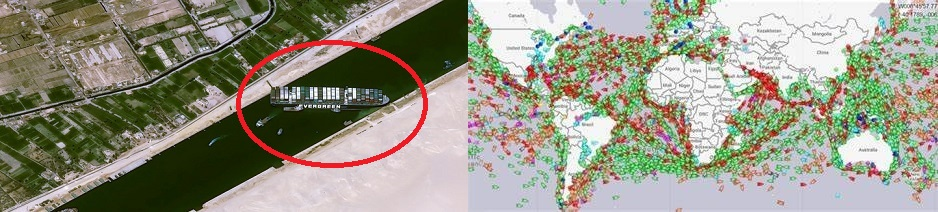
\includegraphics[width=1\textwidth]{evergreen-blockage}
			\caption[Suez canal accident]{Satellite image of Suez canal. On the left showing cargo ship Evergreen stuck in Suez canal in Egypt. The map on the right shows transport ships and freights during the time of the incident (source: FinTechNews.org - 2021). \textit{The colored version shows red spots as all the ships which were affected by the incident}.}
			\label{fig:intro-evergreen-blockage}
		\end{figure}
	
		\subsection{COVID-19 and Patient 31}
		Another interested case comes from public health sector in South Korea. In February 15th, 2020 a 60 year-old patient suffering from novel coronavirus (COVID-19) registered in a health facility in Daegu (150 miles from Seoul, the capital). Having contracted the virus, she continued her visits to a church and a restaurant, thus spreading the disease to other people. By the end of February, her visited church became a disease hot-spot\footnote{Source: https://www.thesun.co.uk/news/11553406/south-korea-patient-31-nhs-track-trace-app}. The magnitude of the spread by this patient alone can be seen in figure \ref{fig:intro-patient-31}.

		\begin{figure}[H]
			\centering
			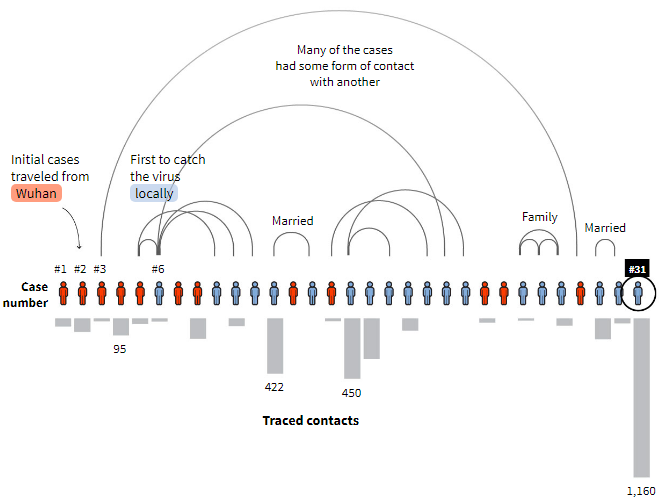
\includegraphics[width=1\textwidth]{patient-31}
			\caption[COVID19 spread in Korea]{Contact tracing graph showing how the novel coronavirus spread from original source in Wuhan to patient 31 (source: Reuters - 2020).}
			\label{fig:intro-patient-31}
		\end{figure}

From the above-discussed case studies, we observe that there are some people, places, or events that seemingly appear insignificant but leave a huge impact on real-world systems. This research is about studying connected systems and relevant methods to identify these impactful people, places, or events. Typically, this entails a small set of individual entities which can effectively spread an action, be it to deliver a piece of breaking news in a social network, market a product to a network of multinational businesses, or place sensors in a sea bed to detect rare species in most probable paths in a network of deep-sea junctions. And this can be done using what this document refers to as \textit{Influence Mining} \footnote{The term "influence mining" was first used by Liu et. al. in 2010\cite{liu2010}}.

Next sections shed light on what networks are and how they can be used to solve the outstanding problem of influence mining.

	\section{What are networks? How can they be used for influence mining?}
	\label{sec:intro-networks}
	Consider a food web\footnote{Ecological food cycle order, which defines what-eats-what.} \cite{cohen1990}, a network of neurons in the brain of a worm \cite{achacoso1991}, global airline routes \cite{guimera2005}, or the World Wide Web \cite{www2015}, all of these unified and connected systems can be represented using Graph theory\footnote{A branch of mathematics, which deals with interactions (edges) between two or more objects (nodes).} in a very simple manner. Each entity can be considered a Node and each interaction between two of such entities can be considered an edge. This formation is generalizable to many domains with numerous applications. Figure \ref{fig:intro-evergreen-blockage} is an example, where the Suez canal is a highly influential edge. Similarly, figure \ref{fig:intro-patient-31} is an example where patient 31 is a highly influential person in the network of her contacts.
	%, and can also be easily scaled.
	
	Graphs or -- referred to from here on as -- Networks are of various types. Regular networks are mathematically constructed and follow a fixed pattern. These networks have lowest heterogeneity (the number of connections each node has are quite uniform) as well as low randomness (meaning that the probability of two nodes to be connected follow a fixed pattern). Some examples of regular networks are:
	
	\begin{enumerate}
		\item Binary trees: A network in which each node has either one or two child nodes. %TODO: Add reference
		
		\item Mesh: Also called grid, is a network in which is graph cartesian product of path graphs on $m$ and $n$ nodes. It is expressed visually as a grid of $n$ rows and $m$ columns. %TODO: Add reference
		
		\item N-regular: A network in which each node has exactly $n$ neighbours, i.e. the degree is same for all nodes. %TODO: Add reference
		
		\item Clique: A type of network in which every node has a direct edge with every other node in the network. %TODO: Add reference
	\end{enumerate}
	
	 Examples of regular networks can be found frequently in engineering, similar to how a computer network can have a star schema in which one node is connected with every other node, forming a star shape. Another example can be a ring of train stations in which each node is connected to exactly two nodes to form a circle. Figure \ref{fig:intro-regular-graphs} shows some examples of regular graphs.
		
	\begin{figure}
		\subfloat[Binary tree]{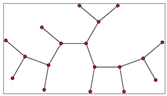
\includegraphics[width=0.3\textwidth]{graph_binary_tree}}
		\subfloat[Mesh graph]{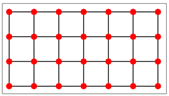
\includegraphics[width=0.3\textwidth]{graph_mesh}}
		\subfloat[$n$-regular graph]{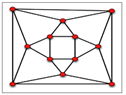
\includegraphics[width=0.3\textwidth]{graph_n_regular}}
		\caption[Examples of regular graphs]{Various types of regular graphs. Each of these are following a fixed pattern of connections.}
		\label{fig:intro-regular-graphs}
	\end{figure}

	Second type of networks are random networks. They are identified by their key property that the probability of connection between any two nodes follows random distribution. Such networks are only generated synthetically, they do not exist in real-world. Famous scientist Albert-László Barabási said:
	
	\textit{We do not know of any real network that is accurately described by the random network model.}\cite{barabasi2016}
	
	However, random networks play a key role in theoretical studies around connected systems. They also provide benchmarks for comparison when real world connected systems are studied for various phenomena.
	
	% They also serve the purpose of starter graphs in order to construct other complex networks \cite{zaidi2013}.
	
	The third type is called Complex networks. In contrast to regular networks, complex networks are highly heterogeneous and have high randomness. The Pareto principal does not apply on regular or random networks because each node in those networks is similar in properties to other nodes; instead, it applies to complex networks where nodes differ from each other in one or more ways.
	
	Complex networks themselves are a broad group, and contain further different types of networks, and because of their relationship with real life scenarios, the area of complex network analysis has caught attention in the last few decades. From neural networks in a human brain to a social network of professionals, an Intranet of computers to Internet of things, and network of food delivery riders to global networks of airways, the applications where complex networks can be found are limitless. The examples given in \ref{sec:intro-global-events} are a few cases of complex networks: the Iceland volcano eruption is a case based on a network of airways; the Suez canal blockage is an example from global sea trade industry; patient 31 is a case from a contact tracing network in epidemiology.
	
	It is not trivial to study complex networks in a generic view, they are studied on at least three levels: micro-scale, which focuses on individual nodes; meso-scale, an intermediate level which deals with entities like clusters and groups; macro-scale, where the network is analyzed as a whole. As a result, such networks hold some properties for which, conventional techniques of studying them are no longer applicable; this opens new gates of exploration for us. Some commonly observed examples include scale free structure \cite{barabasi1999}, in which the degree distribution of the nodes follow Power-law (as shown in figure \ref{fig:intro-scale-free-network}; small-world property \cite{watts1998} in which the nodes have high number of triads\footnote{A complete graph of three nodes in a network.} and small average path length (APL)\footnote{Average minimum number of edges required to travel from one node to the other.} (figure \ref{fig:intro-small-world-network} is an example); community structure \cite{strogatz2001} where cluster-like sub-networks can be observed within a large network; high tolerance (resilience) \cite{albert2004}, where the network does not collapse or change its structure if a few random nodes are removed. These three levels are not completely segregated, they overlap each other. Thus it is vital to analyze a complex network holistically as well as on granular scale.
	

	\begin{figure}[H]
		\centering
		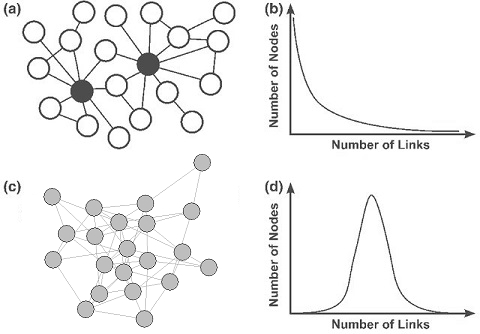
\includegraphics[width=0.75\textwidth]{scale-free-network}
		\caption[Scale free network]{Diagram 'a' shows a scale free network with some vital nodes highlighted; diagram 'b' shows the distribution of node degrees of the scale free network; diagram 'c' is a random network; diagram 'd' is the distribution of node degrees of the random network (attribution: Ilya-Temkin - ResearchGate.com).}
		\label{fig:intro-scale-free-network}
	\end{figure}
	
	\begin{figure}[H]
		\centering
		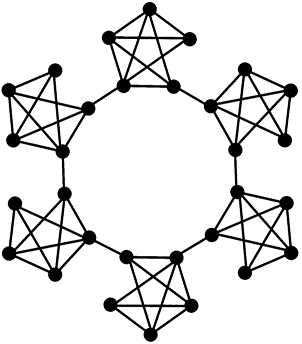
\includegraphics[width=0.5\textwidth]{small-world-network}
		\caption[Small-world network]{Watts and Strogatz model of small-world networks. Given example is generated by rewiring a lattice (regular network).}
		\label{fig:intro-small-world-network}
	\end{figure}
	
	Some advanced types of complex networks also include heterogeneous networks in which nodes and/or edges can be of multiple types (see figure \ref{fig:intro-heterogeneous-network}, and evolving networks which change their shape over time like the one shown in figure \ref{fig:intro-evolving-network}. The aforementioned examples only scratch the surface. The stack of known complex network types is thick, Costa et. al \cite{costa2011} thoroughly discussed a variety of complex networks and their applications in 22 ways. As specified in \ref{chp:domain}, it is beyond the scope of this study to discuss each type of complex network.
	
	\begin{figure}[H]
		\centering
		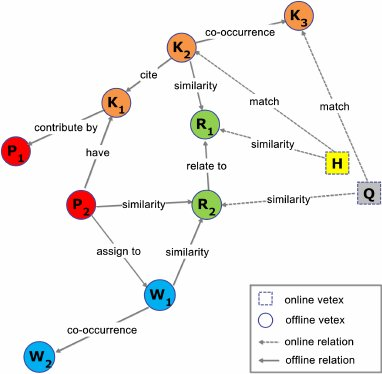
\includegraphics[width=0.5\textwidth]{heterogeneous-network}
		\caption[Heterogeneous network (OER)]{Heterogeneous network of Open Educational Resource based collaboration (attribution: Xiaozhong Liu \cite{liu2015b}). There are two types of nodes, online and offline as well as two types of relationships, i.e. online and offline.}
		\label{fig:intro-heterogeneous-network}
	\end{figure}
	
	\begin{figure}[H]
		\centering
		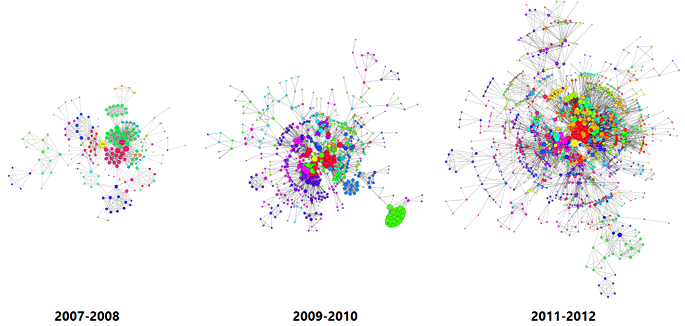
\includegraphics[width=1\textwidth]{evolving-network}
		\caption[Evolving network of Apple Inc.]{Inventor network of Apple Inc. Each node is an inventor, and an edge shows a collaboration of a patented invention.}
		\label{fig:intro-evolving-network}
	\end{figure}


	\section{Social networks: a use case of complex networks}
	\label{sec:intro-social-networks}
	Among all common complex networks, social networks are very well studied across a spectrum, ranging from a handful of students to the largest network of social ties in the 21st century, Facebook – connecting over 1 billion people. Social networks exhibit the properties of complex networks, i.e. they are scale free as well as small-world, contain community structures, are heterogeneous, and exhibit more unique properties than any other class of network. A social network may consist of following components, which shall be discussed later as required:
	
	\begin{itemize}
		\item Platforms including Social Networking, Blogging/Micro-blogging, Content Sharing, Message Boards, Chat Rooms, Podcasts, RSS Feed and Web Widget \cite{cui2011}.
		
		\item Active participants. These are typically the nodes in social network.
		
		\item Information generated and shared between users. This information is in form of transaction logs, a term used by researchers; such logs are usually in form of structured database, not in a graph form.
		
		\item Relations between users like Friend, Family, Co-worker, Acquaintance, etc. These relations are represented as edges in the social network. Some researchers have used the term "link" instead of "edge".
	\end{itemize}
	
	Thus, a prime example of complex network analysis is studying correlation \footnote{Discovering patterns by analyzing actions performed by pairs of nodes in a network.} between nodes in a large social network, in which people are connected to each other in various manners, making it harder to understand the nature and the cause of relationship between them. To understand this concept better, imagine five customers shopping for a flower pot in a nursery. First customer buys a lavender plant; of the rest of the customers, three more also buy a lavender pot. How did this happen? If we rule out coincidence, then the logical conclusion would be that there is some kind of \textit{correlation} in buying patterns between these four customers, which does not match with the fifth customer. From here, we can draw three conclusions:
	
	\begin{enumerate}
		\item All four customers like scent and colour of lavender flower, and bought them out of their own liking. In this case, the correlation is their personal preference.
		
		\item They live in same neighbourhood where mosquito are common, and lavender scent is a good repellent of mosquito. Therefore, they did not buy due to personal liking but rather the correlation between their purchase were confounding factors.
		
		\item The first customer inspired other customers to buy the same plant. In this case, neither personal preference nor confounding factors were involved. Such source of correlation is called influence.
	\end{enumerate}
	
	Anagnostopoulos has explained these correlation sources in detail \cite{anagnostopoulos2008}. In the same fashion -- as the use case of social networks -- an example from complex networks can be transportation networks, where the airports/sea ports can be considered as nodes and direct flights/sea routes between them can be edges. This network grows as newer logistic corridors are formed between countries, shaping into a complex network. Recalling from example of Suez canal blockage, the network shown in figure \ref{fig:intro-evergreen-blockage} illustrates the tens of thousands of cargo ships sailing from one port to another, the ports in this case are nodes while the route these ships follow are edges. Ports can be connected with each other either directly, or via a path. The objective of discovering influential nodes in such networks is fundamentally similar to social networks \cite{rocha2017}. \\
	
	\section{Application areas}
	\label{sec:intro-applications}
	The spectrum of applications of influence mining is broad. A holistic method to describe several application areas will be that any problem which can be mathematically modeled as a graph such that the nodes of the graph describe entities and edges define the relationships between these entities, and that the objective of the problem is to identify vital or influential entities and/or super spreaders which have the potential to impact other entities and their relationships, can be studied as a use case of influence mining. We further discuss a few application areas as follows:
	
		\subsection{Viral marketing}
		One of the widest applications of social influence is in the field of viral marketing. The concept behind viral marketing is to promote an idea, a product or news in a network of people by finding influential nodes; this way, with a minimal marketing cost, the marketing objectives can be achieved, i.e. spreading the idea, product to a large part of a social network \cite{tang2017,talukder2018}.

		\subsection{Outbreak detection}
		Outbreak detection is selecting nodes in a network to detect and prevent the spread of a virus or malware in order to minimize damages. This is another application with wider reach as it can be applied to many domains where an event can cause a ripple effect mutilating an entire network \cite{balthrop2004}. The examples of Northeast power outage and Patient 31 of COVID19 virus discussed in section \ref{sec:intro-global-events} are both cases of outbreak detection.
		
		\subsection{Recommender systems}
		Online social networks have become very popular in the past few years with billions of visitors each day. There are various applications of influence maximization in social networks such as Twitter and Facebook \cite{banerjee2020}. For example, application of recommendation systems in which the goal is to recommend the right products and utilities to a user based on the transaction log of his close network \cite{cai2020}, who are likely to influence this user to buy those products. Such applications require high-quality data on various personality traits, locale details and transaction trails. Moreover, due to growing concerns on information privacy \cite{kayes2017}, it is becoming harder to collect and keep user data. With the help of influence mining, such challenges can be overcome as the data requirements are reduced to network information and transaction logs.
		
		\subsection{Economy}
		Financial markets, especially with the emerging boom of crypto-currencies, which in principal, are based on block chain networks make full use of influence mining. For example, a block chain has two types of nodes: full and partial. Partial nodes are light nodes which carry only a proportion of transaction logs, however s complete ledger is maintained on each of the Full nodes, which is not only responsible for keeping all data \footnote{As of November 2021, the ledger size of crypto-currency block chain has grown to 366GB in size. Source: https://www.blockchain.com/charts/blocks-size}, but also verify all the \textit{blocks} (a collection of verified transactions). This entails high costs of computation power, electricity consumption, and personnel to manage. The more such full nodes are added to block chain, the more time it takes to verify blocks. Influence mining can be particularly handy to identify the minimal set of full nodes to keep the block chain efficient as well as robust. In fact, it can be argued that since financial data is more reliable and accurate as compared to other fields \cite{costa2011}, influence mining is likely to be more effective if we model their instruments, business ties, investors, consumers, etc. as a network. Chapter \ref{chp:inf-max} presents an experiment on a real economic network as a case study of influence mining application. \\
	
	Moreover, the influence mining can be applied in the field of Epidemiology, especially public health for example to control a contagious disease; in Electronics to optimize a large circuit; in ecology to learn predator-pray relationships; in neuroscience to monitor the activity of brain receptors during various events; in tourism to determine the most favorable paths and destinations in order to provide best tour packages. Numerous other application areas can identified thus making this a very interesting field of study.


	\section{Why influence mining?}
	We have presented several examples from the real life where identifying influential nodes in a network can be very useful. The crucial question here is to answer whether influence mining is the right approach or not?
	
	Let us pick the first examples we discussed in section \ref{sec:intro-global-events}. The volcano eruptions from Eyjafjallajökull peak caused giant cloud of smoke and ash, thus resulting in blocking all flights routed to not only Iceland, but also through Greenland. For most of these flights, the desired destination was neither Iceland, nor Greenland but rather USA and Canada. However, due to convenience of flying near land, many of the flights transit through Iceland. The map in figure\ref{fig:europe-iceland-flights} shows that there's only one airport, i.e. Iceland's Keflavik airport, which was a destination to more than 50 flights. All the other airports seem to be less relevant. The process of influence mining would have predicted not only Keflavik, but other potential influential routes for airways, which could have been used as alternate paths in case of unavailability of Keflavik.
	
	\begin{figure}[h]
		\centering
		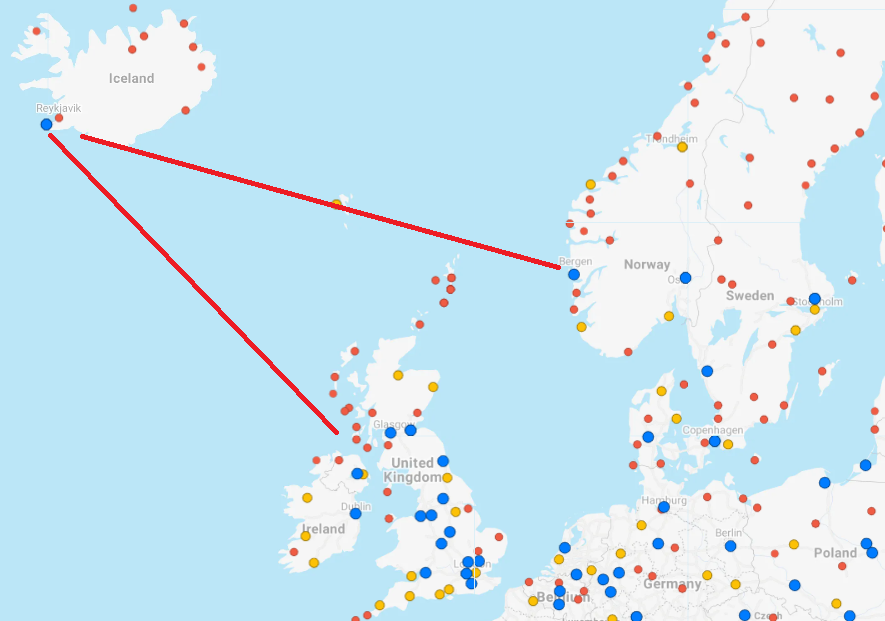
\includegraphics[width=1\textwidth]{europe-iceland-flights}
		\caption[Europe to Iceland flights]{Snapshot of European airports showing destinations. Large (blue) pins are the airports where more than 50 flights land, while small (red) circles are the airports hosting 10 or less flights (Source Flight connections - 2021).}
		\label{fig:europe-iceland-flights}
	\end{figure}
	
	Similarly, in case of Coronavirus spread from Patient number 31, the strategy of disease outbreak control followed standard contact tracing practices, i.e. start with the infected person, then trace the close contacts within 1-degree \footnote{Degree of a node is the measure of edges or links with other nodes in a network.} distance, then follow the contacts within 2-degree distances. This approach of disease transmission analysis and control is exponential and very soon makes it impossible to screen all the susceptible people. On the other hand, influence mining solution inputs a network and identifies all potential spreaders at once, thus minimizing the screening effort as well as enhancing efficiency of field workers. With application of such strategy, Patient 31 could have been identified as potential spreader much earlier \cite{dong2020}. \\

Concisely, the problem of analyzing complex network such as social networks, can therefore also be studied as a case of influence mining, which is the process of finding a set of people, places and events in a network which can independently as well as collectively influence rest of the nodes in a network to perform certain action, or respond to an action. It's important to note that there are multiple terms used in the literature to represent the same notions: "influential nodes" are also referred to as "vital nodes","super spreaders", "important nodes" or "critical nodes"; the problem of "influence mining" is originally called "influence maximization" \cite{kempe2003}, "nodes" are known as "vertices" in some studies, "edges" can also be termed as "links" or "relations". However in the next chapter we will discuss why the term "mining" is connected with the presented work, and is therefore preferred in this document.
